\chapter{The Power of Ambition}

This chapter follows Jim Rohn's lecture as preserved in the LazyingArt LLC curation of the Jim Rohn originals. The lecture opens by asking us to listen, take notes, and cultivate the ideas rather than merely admire them, and that overture matters. What follows is not a neutral taxonomy but a guided practical argument. Its formal spine is structural rather than algebraic: definition chains, numbered principles, allocation rules, feedback loops, and measurable checkpoints. We therefore keep the spoken order. First the lecturer clears moral ground; then he sharpens the meaning of ambition; then he gives it motivational force through dreams, examples, and repeated resolve; only after that does he step back and unfold the daily mechanics.

\section{Ambition, Greed, and Disciplined Desire}

We begin where the lecture begins: with a restriction. Ambition is introduced as powerful, but not morally free. It is permitted only under a discipline of service.

\begin{definition}
\[
\text{legitimate ambition} := \text{ambition at the service of others, not at the expense of others}.
\]
\end{definition}

This is not decoration around the subject. It is the first condition of the subject. The lecture returns to it whenever health, wealth, power, and success come into view.

The lecturer then moves from dictionary language to an operational definition. The crucial distinction is not yet between high ambition and low ambition, but between wanting and the kind of wanting that actually acts.

\begin{definition}
\[
\text{true ambition} := \text{disciplined eager desire}.
\]
\end{definition}

The opening chain can therefore be written in compact form:
\begin{equation}
\text{wish} \to \text{desire} \to \text{disciplined eager desire} = \text{ambition} \to \text{daily action} \to \text{changed life}.
\end{equation}
Desire names the wanted end. Ambition names the disciplined route to that end:
\begin{equation}
\text{desire} := \text{wanted end}, \qquad
\text{ambition} := \text{disciplined process that reaches it}.
\end{equation}

\paragraph{A worked chain.}
The lecture's first derivation is conceptual, but it is exact enough to lay out step by step:
\begin{enumerate}
\item A wish names a hoped-for change.
\item The wish must harden into desire.
\item Desire without discipline stalls.
\item Discipline turns eager desire into ambition.
\item Ambition requires action today, not admiration tomorrow.
\item Repeated daily action changes the shape of a life.
\end{enumerate}
This is why the lecture immediately gives ordinary examples. If we want to be ready for a meeting tomorrow, we prepare today. If we want to pay for a child's education, we save today. If we want a better life tomorrow, we work on it today. Ambition is not a mood. It is a minute-by-minute and day-by-day mentality.

\subsection{Question \& Answer}

\paragraph{Is ambition just greed in respectable language?}
No. The lecture is emphatic on this point. Greed is gain by injury, manipulation, or destruction. Ambition, by contrast, is constructive. It wants the larger house, the stronger business, the healthier body, or the wider influence by becoming worthy of them and by serving others in the process. This is why the lecture pauses over Judas: money may be acquired without success, and gain may be secured without peace. The moral distinction is therefore built into the definition itself.

\section{Dreams That Pull and Principles That Organize Life}

Having separated ambition from greed, the lecture asks its next question: what gives ambition enough force to last? The answer is not bare wanting but vivid futurity. The successful are pulled; the merely wistful remain where they are.

\begin{equation}
\text{fuzzy future} \Rightarrow \text{little pull}, \qquad
\text{vivid dream} \Rightarrow \text{strong pull}.
\end{equation}

A dream, in the lecture's sense, is a projection of the life we want to lead. Once that projection becomes vivid, it does more than console. It reorganizes the present. The lecture does not state this as an abstraction first. It states it by image and story: pioneers crossing mountains, immigrants arriving with little, and the repeated demand that we see the finish before we stand at the finish.

\paragraph{Anecdote and motive.}
The lecturer asks us to imagine settlers climbing the mountains while already seeing California on the other side. He asks us to imagine immigrants who arrive with less but possess a defined goal and therefore often build more. The point is not sentimental. The point is causal. When the mind sees the future finished in advance, the present becomes more bearable. And once a person is willing to do the uncomfortable until it becomes comfortable, ambition acquires temporal depth.

The lecture then turns from example to quasi-formal summary by attributing to Franklin a three-part schema:
\begin{equation}
F_{\text{Franklin}} := (\text{small daily advantages},\ \text{life is moldable},\ \text{success as pleasure in present activity}).
\end{equation}
The first point guards us from waiting for one giant victory. The second point restores agency: life is not fixed but worked upon. The third point corrects a common error. Success is not only the possession at the end. It includes the right pleasure in the work now.

Next the lecture attributes to William James a two-part account of success:
\begin{equation}
J_{\text{James}} := (\text{inner ideal pursued persistently with courage},\ \text{outer achievement related to that ideal}).
\end{equation}
The order matters. The lecture lingers over the first part. Read the books until the skill changes. Go to the seminars until the thing makes sense. Practice until you can do it. Here the repeated word \emph{until} is not ornament. It is the time-form of resolve.

Only after this rise through dreams, pioneers, immigrants, Franklin, and James does the lecture step back and name its main architecture:
\begin{align}
P_6 := (&\text{positive self-direction},\ \text{self-reliance},\ \text{self-discipline}, \nonumber\\
&\text{self-enterprise},\ \text{working with others},\ \text{self-appreciation}).
\end{align}
This recap is important. It prevents the middle of the lecture from dissolving into scattered advice. We are now meant to hear the next long stretch as an ordered unfolding.

\subsection{Question \& Answer}

\paragraph{What turns a wish into a force that can organize a life?}
The lecture's answer has three parts. First, the future must be vivid enough to pull. Second, the future must be broken into daily advantages and daily disciplines. Third, the will must consent to duration; it must keep going \emph{until}. Wish by itself has no temporal stamina. Dream plus discipline does.

\section{Positive Self-Direction: Knowing Ourselves and Preparing Ourselves}

The first principle in the long middle stretch is positive self-direction. Here the lecture becomes more diagnostic. The question is not only where we would like to go, but whether the disciplines we are now living by are taking us there.

\begin{equation}
\text{positive self-direction} := (\text{self-knowledge},\ \text{self-preparation}).
\end{equation}

The keynote is simple and stern:
\begin{equation}
\text{direction} \Rightarrow \text{destination}.
\end{equation}
The lecturer repeats the question in several forms because he does not want us to evade it. Are the present disciplines really taking us toward the desired destination, or are we merely hoping while moving elsewhere?

\paragraph{Self-knowledge.}
Self-knowledge means more than listing goals. It means knowing who we are, what sort of life is genuinely ours, what our present attitudes are doing to us, and whether the ambition we carry belongs to us or has been borrowed from family, class, or profession. The lecture includes a severe example here: the story of a woman raised inside a medical-family tunnel who later discovered that the goals she had pursued were not her own. In the lecture's telling, the cost of mistaken direction can be psychic and even bodily. A direction that is not ours may still be impressive; it may also be damaging.

This is why the lecture asks its hardest inward question here rather than later:
\[
\text{Is it mine?}
\]
That question applies not only to career but also to style, method, and the very picture of success itself.

\paragraph{Self-preparation.}
Preparation means becoming ready before the opportunity arrives. The lecture gives this a definite three-step form:
\begin{equation}
\text{self-preparation} := (\text{consider resources},\ \text{determine concrete preparation},\ \text{increase likelihood of opportunity}).
\end{equation}
In words, we first ask where the next opportunity is likely to originate. Then we specify what concrete preparation is required. Finally we do additional work to make the opportunity more likely to occur.

No lecture-frame diagram survives for this section, so the following schematic is an editorial reconstruction from the transcript alone.

\begin{figure}
\centering
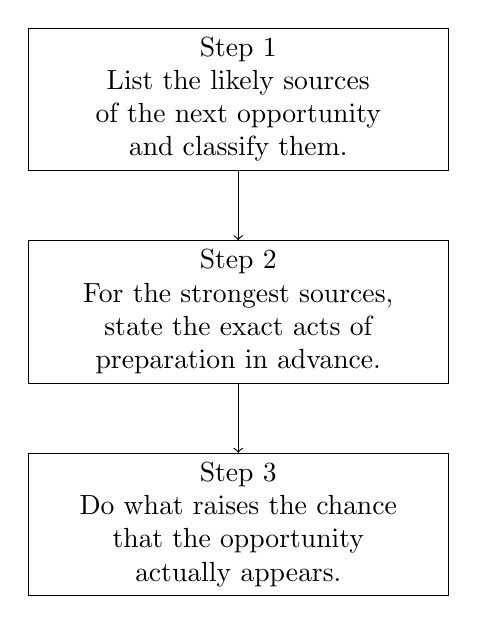
\begin{tikzpicture}
\node[draw, align=center, text width=5.1cm] (a) at (0,0) {Step 1\\List the likely sources\\of the next opportunity\\and classify them.};
\node[draw, align=center, text width=5.1cm] (b) at (0,-2.7) {Step 2\\For the strongest sources,\\state the exact acts of\\preparation in advance.};
\node[draw, align=center, text width=5.1cm] (c) at (0,-5.4) {Step 3\\Do what raises the chance\\that the opportunity\\actually appears.};
\draw[->] (a.south) -- (b.north);
\draw[->] (b.south) -- (c.north);
\end{tikzpicture}
\end{figure}

The lecture even supplies a classification language: some resources are sure things, some good bets, some even chances, some unlikely, some long shots. What matters is not numerology. What matters is that hoping becomes ranked preparation.

The lecture also states two benefits of preparation:
\begin{align}
\text{self-preparation} &\to \text{movement toward the goal},\\
\text{self-preparation} &\to \text{renewed ambition through present activity}.
\end{align}
Activity now is not only means; it is fuel.

At the end of this section the lecture compresses a worthwhile life into four terms:
\begin{equation}
\text{worthwhile life} := (\text{learn},\ \text{try},\ \text{stay},\ \text{care}).
\end{equation}
The order is exact. We learn, then try; we stay long enough for the attempt to become real; and we care enough for the process to keep its force.

\subsection{Question \& Answer}

\paragraph{Are these goals really mine, or am I living inside someone else's plan?}
The lecture's answer is not quick reassurance. We must ask, debate, compare, and write until the goal has survived inspection as our own. An inherited goal can produce impressive motion and inner damage at the same time. Positive self-direction therefore begins with ownership of direction, not merely with effort.

\section{Self-Reliance and Self-Discipline as the Missing Link Between Knowledge and Results}

Once direction is chosen, the lecture turns to friction. Why, after all the books, seminars, plans, and good intentions, do we still fail to move? Here the lecture joins the second and third principles: self-reliance and self-discipline.

Self-reliance is not isolation. It is responsibility. What is happening to us now is tied, in the lecturer's practical sense, to what we did yesterday. That does not mean every event is self-caused. It means improvement does not begin with blame. If we do not take charge of reading habits, skills, effort, follow-up, and preparation, the hoped-for destination does not arrive by courtesy.

The lecture then gives one of its clearest operational definitions:
\begin{equation}
\text{discipline} := \text{awareness of need for action} + \text{conscious implementation now}.
\end{equation}
The companion definition is equally sharp:
\begin{equation}
\text{procrastination} := \text{delay between awareness and implementation}.
\end{equation}
This is a genuine decision rule. If awareness and implementation coincide, the sequence is discipline. If a gap opens between them, the sequence becomes procrastination.

\subsection{Question \& Answer}

\paragraph{If knowledge is power, why do we still fall short?}
Because knowledge unused is not yet power in the life. The lecture insists on a sequence: apply what we know, study the result, refine the approach, and apply again. The missing link is not usually the next seminar. It is consistent self-discipline.

The lecture then states the positive reinforcement loop in nearly formal form:
\begin{equation}
\text{disciplined action} \to \text{small result} \to \text{positive reinforcement} \to \text{stronger habits} \to \text{more disciplined action}.
\end{equation}
This loop matters because it explains how ambition becomes easier to sustain. It is not sustained by slogans alone. It is sustained by visible return.

The lecture also offers one of its most memorable paired formulas:
\begin{equation}
\text{easy to do} = \text{easy not to do}.
\end{equation}
That is why neglect is dangerous. The first day rarely punishes it. The disaster appears only after long repetition. Hence the paired contrast:
\begin{align}
\text{few disciplines every day} &\to \text{fortune},\\
\text{few errors every day} &\to \text{disaster}.
\end{align}

\paragraph{Writing, tracking, and planning.}
At this point the lecture repeatedly asks us to take thought out of vapor and put it on paper. Journal the day. Write out the problem. Reflect on the week. Develop the game plan. The formal summary is compact:
\begin{equation}
\text{game plan} := \text{Activities} \times \text{Days / time blocks}.
\end{equation}
This is the graph-paper method. We do not start the day until we have it finished. Then we do the same for the week and for the month. The point is not bureaucracy. The point is that visible structure helps ambition survive low-energy days. Each task is seen as a link in a chain rather than as a lonely burden.

\section{Self-Enterprise and Working With Others Without Losing Moral or Strategic Clarity}

The next movement begins with self-enterprise. Discipline by itself can become passive if it only protects routine. Enterprise adds initiative. It creates opportunity instead of waiting for it. But the lecture does not allow enterprise to become isolation. As soon as the inward machinery is built, it must prove itself in the company of other people.

\paragraph{Self-enterprise.}
The lecture first treats enterprise as creativity plus courage plus prepared action. The enterprising person sees a sculpture in scrap metal, a housing development in a ruined neighborhood, a secondary market where others see none, and a future use in a present fragment. Just as important, the enterprising person is willing to act on such perceptions.

The lecture then gives a practical problem-solving triad:
\begin{equation}
\text{problem solving} := (\text{What can I do?},\ \text{What can I read?},\ \text{Who can I ask?}).
\end{equation}
The order matters. We first attack the problem directly. Then we search the written record of others. Only then do we ask for help, and when we ask, we bring working papers with us. Thought on paper is repeatedly preferred to thought trapped in fog.

The lecture extends this inventive discipline through brainstorming, outlandish solutions, doodles, flowcharts, and formulas. The common point is that the mind must be shaken out of ruts. Some ideas are valuable precisely because they are initially impractical; they loosen the grip of the obvious.

\subsection{Question \& Answer}

\paragraph{How do we create opportunity instead of merely waiting for it?}
The lecture's answer is procedural. Think on paper. Ask what can be done, then what can be read, then whom to ask. Brainstorm without premature censorship. Consider even the absurd. Use diagrams and doodles if they wake another part of the mind. Enterprise is not luck. It is prepared alertness kept active.

\paragraph{Inner enemies.}
The courage half of enterprise is equally important. Here the lecture names the enemies that must be fought on the inside: fear, indifference, indecision, doubt, worry, and over-caution. These are not incidental moods. They are thieves of opportunity. The enterprising person must therefore do battle not only with outer obstacles but with inner hesitation.

The lecture then turns outward. Working with others is not a retreat from self-reliance. It is the necessary proof that self-reliance has matured. We cannot be successful by ourselves. The lecture states this bluntly and often.

\paragraph{Communication and relation.}
Kindness, sensitivity, good questions, sincerity, repetition, brevity, style, vocabulary, and reading the audience are all presented as productive skills. We are told to express rather than impress. We are told to read what we see, what we hear, and even what we feel in the encounter. Good communication is not ornamental polish. It is a discipline that builds trust and therefore makes ambitious action socially effective.

When criticism is necessary, the lecture recommends distinction rather than confusion: condemn the deed, not the person. In one reported rule of thumb:
\begin{equation}
\text{kind criticism} := 3 \text{ appreciations} + 1 \text{ correction}.
\end{equation}
This is not sentimental softness. It is a way of making correction usable rather than merely explosive.

Networking is treated in the same moral-practical register. Keep the relation active, be grateful, make it mutually beneficial, do not call only when you need something, and remember that appreciation is not lost when given; it is invested.

The lecture's older maxims belong here:
\begin{equation}
\text{if you wish to receive} \Rightarrow \text{you must give},
\qquad
\text{if you search} \Rightarrow \text{you find}.
\end{equation}
And even more sharply:
\begin{equation}
\text{if you plant} \Rightarrow \text{you reap}, \qquad
\text{need alone} \not\Rightarrow \text{reap}.
\end{equation}
These are not finance theorems. They are practical laws of self-management as the lecture presents it.

The same outward turn reaches family life. Communication at the dinner table, activity together, compatible rules across households, and deliberate attention to children and spouse are not optional soft themes attached to the real material. They are part of the real material. Work and home affect one another. Everything affects everything else.

\subsection{Question \& Answer}

\paragraph{How can ambition be self-reliant and still depend on other people?}
Because self-reliance is not solitude. It means taking responsibility for the value we bring. Once that value exists, it must move through relation: clients, colleagues, children, spouse, friends, associates. The lecture's formula is simple: each of us needs all of us. Ambition remains personal in origin, but relational in realization.

\section{Self-Appreciation, Financial Independence, and Measurable Progress}

The sixth principle is self-appreciation. Here the lecture slows down long enough to prevent ambition from becoming one more form of blind self-rejection. We are told to acknowledge what has been done, to enjoy the plateau, and to refuse the stereotype that success must look the same for everyone.

\paragraph{Self-appreciation.}
Success, in the lecture, has no single costume. It is not reducible to the standard salary, the standard address, or the standard car. The lecturer is explicit:
\begin{definition}
\[
\text{success} := \text{steady progress toward your own personal goals}.
\]
\end{definition}
This is why self-appreciation matters. It keeps us moving by letting present gains feed future effort. It is not vanity. It is accurate acknowledgment.

The finance discussion therefore arrives as a continuation of this point, not as a separate doctrine. If wealth is part of our chosen destination, the lecture insists that it is acceptable to want it, provided the moral restriction is preserved.

\begin{definition}
\[
\text{financial independence} := \text{the ability to live from the income of one's own personal resources}.
\]
\end{definition}

The lecturer then gives the chapter's clearest arithmetic rule:
\begin{equation}
\text{spend} \le 0.70Y,\qquad
\text{charity}=0.10Y,\qquad
\text{active capital}=0.10Y,\qquad
\text{passive capital}=0.10Y.
\end{equation}
Here \(Y\) denotes income. The order matters philosophically. The rich, as the lecture puts it, invest first and spend what is left; the poor spend first and wonder what disappeared.

\paragraph{Worked example.}
If our monthly income is \(Y=\$5000\), the rule becomes
\begin{align}
\text{spending} &\le 0.70Y = \$3500,\\
\text{charity} &= 0.10Y = \$500,\\
\text{active capital} &= 0.10Y = \$500,\\
\text{passive capital} &= 0.10Y = \$500.
\end{align}
The lecture presents this as practical philosophy, not as formal financial advice. Its force lies in repeated discipline, strict accounts, and time.

The same section sharpens measurement. We are not to live by vague stories about progress. We are to count. The lecture's measure is:
\begin{equation}
\text{measure of success} := \text{measurable progress in reasonable time}.
\end{equation}
The windows of review are themselves structured:
\begin{equation}
W_{\text{results}} := (\text{end of day},\ \text{end of week},\ \text{last 90 days},\ \text{last 6 months}).
\end{equation}
And the sample quantities are concrete:
\begin{equation}
M_{\text{check}} := (\text{money saved and invested},\ \text{books read in 90 days},\ \text{classes taken in 6 months}).
\end{equation}

One of the lecture's cleanest examples comes from sales. If a new salesperson is supposed to make ten calls in the first week, the manager asks on Friday for a number, not for a story:
\begin{equation}
n_{\text{calls}}^{\text{target}} = 10.
\end{equation}
The point is not harshness. The point is that numbers reveal the real relation between intention and result. The lecture says, in effect, that the numbers tell the story.

\subsection{Question \& Answer}

\paragraph{Is it acceptable to want wealth, and how do we measure whether we are truly progressing toward it?}
Yes, if the pursuit remains at the service of others rather than at their expense. And we measure progress by results taken at reasonable intervals. We do not measure it by mood, costume, or stereotype. We measure it by what has actually been saved, learned, built, improved, or completed.

\section{Failure, Patience, Persistence, and the Final Compression Into Character}

Once success has been defined, the lecture performs a necessary reversal and defines failure just as carefully. This is where the argument becomes most protective against discouragement.

\begin{definition}
\[
\text{failure} := \text{not trying} = \text{no progress because one has ceased to act}.
\]
\end{definition}
This matters. A project that did not work is not yet failure if it was honestly attempted, studied, and revised. The lecture reserves the word \emph{failure} for the stoppage of trying.

The lecturer then adds two temporal virtues:
\begin{equation}
\text{persistence} := \text{patience in action}.
\end{equation}
Patience handles the passing of time; persistence keeps action alive during that passing. The lecture refuses to let ambition collapse into impatience. Time is not an insult to the goal. It is part of the price of the goal.

\subsection{Question \& Answer}

\paragraph{What should we do when progress fails, stalls, or takes much longer than we hoped?}
The lecture's answer is plain: do not call the delay final. Study the setback, take responsibility for your part, keep preparing, and continue until. Delay is not refutation. It is often the condition of valuable achievement.

The lecture then broadens failure into adversity more generally. Sometimes one turns around by disgust: \emph{I've had it. Enough. No more. Never again.} That rhetoric is not merely emotional excess. In the lecture it names the moment when passive suffering turns into active resolve. A temporary condition is re-read as material.

Resilience is the name of that re-reading:
\begin{equation}
\text{resilience} := \text{ability to recover after setback}.
\end{equation}
The lecture later expands resilience into a seven-part practical list:
\begin{equation}
R_7 := (\text{insight},\ \text{independence},\ \text{ties to others},\ \text{initiative},\ \text{creativity},\ \text{humor},\ \text{morality}).
\end{equation}
These terms are not arbitrary. Insight examines the loss honestly. Independence refuses paralysis. Ties to others renew motive. Initiative begins again. Creativity finds a new path. Humor prevents collapse into solemn despair. Morality preserves the original ethical boundary: rebound itself must remain at the service of others.

One of the lecture's strongest late formulas then appears:
\begin{equation}
\text{success attracted} \leftarrow \text{the person you become}.
\end{equation}
We do not simply chase success as if it were a butterfly. We become the sort of person capable of attracting and sustaining it.

Only now does the lecture perform its final compression:
\begin{equation}
P_6 \to C_3, \qquad
C_3 := (\text{concentration},\ \text{resilience},\ \text{integrity}).
\end{equation}
This is the mature form of the whole chapter. The six principles, worked on together and every day, become the three cornerstones that stabilize ambition.

Concentration keeps attention where it belongs:
\[
\text{wherever you are, be there}.
\]
Resilience keeps us from surrender after setback. Integrity keeps the whole project morally and personally unified. The lecture's account of integrity is practical and severe:
\begin{equation}
\text{integrity} \Rightarrow \text{pay fair price for fair value, finish what you begin, keep the faith}.
\end{equation}
The lecture's late insistence on fair price, finishing the task, and keeping faith with family, enterprise, and community is not a separate sermon. It is the final protection against ambition becoming corrosive.

This is what prepares the last decisive reversal:
\[
\text{you are more than your ambition}.
\]
Ambition must serve the strengthened self. If we serve ambition instead, we become smaller than the instrument we meant to use.

\section{Summary}

The lecture unfolds in a deliberate order. It begins not with appetite but with ethics: ambition is legitimate only at the service of others. It then distinguishes wish, desire, and disciplined eager desire, and gives ambition its pull through vivid dreams, pioneers, immigrants, Franklin, James, and the repeated discipline of \emph{until}. Only after that crest does it step back and name the six principles: self-direction, self-reliance, self-discipline, self-enterprise, working with others, and self-appreciation.

From there the chapter becomes increasingly operational. Goals must be our own. Preparation must be concrete. Knowledge must be applied. Problems must be worked on paper. Time must be planned. Money must be allocated. Progress must be counted. Failure must be re-read as stoppage of trying rather than as temporary defeat. At the end, the six principles compress into concentration, resilience, and integrity. Those three give stability to ambition, and stability is what lets ambition remain an instrument of growth rather than a master of the self.